\section{Guida all'installazione}
Per lo sviluppo del Back-end del progetto è stato utilizzato l'IDE di sviluppo Visual Studio Code e per la programmazione del Front-end l'IDE Android Studio. Il Database risiede su Amazon AWS. 
\subsection{Installazione Android Studio}
\begin{enumerate}
    \item Andare sul sito \textit{https://developer.android.com} e cliccare sul bottone \textit{Download Android Studio}. Figura \ref{fig:installazione1}
    \item Accettare i termini e le condizioni e premere il bottone \textit{Download Android Studio}. Figura \ref{fig:installazione2}
    \item Aprire il file eseguibile. Figura \ref{fig:installazione3}
    \item Se presenti vecchie versioni di Android Studio verrà chiesta la conferma per cancellarle. Cliccare \textit{Next}. Figura \ref{fig:installazione4}
    \item Cliccare \textit{Next} per continuare con l'installazione. Figura \ref{fig:installazione5}
     \item Cliccare \textit{Next} per continuare con l'installazione. Figura \ref{fig:installazione6}
     \item Scegliere la cartella di installazione e cliccare \textit{Next}. Figura \ref{fig:installazione7} 
     \item Scegliere la cartella dove verranno salvati i programmi e cliccare  \textit{Install}, una volta conclusa l'installazione cliccare  \textit{Next}. Figura \ref{fig:installazione8} 
     \item Cliccare il bottone  \textit{Finish} per terminare l'installazione e far avviare l'IDE. Figura \ref{fig:installazione9}
\end{enumerate}

\begin{figure}[htbp]
    \includegraphics[width=\textwidth]{guida-installazione/android-studio/1.PNG}
    \centering
    \caption{Installazione Android Studio - Fase 1}
    \label{fig:installazione1}
\end{figure}

\begin{figure}[htbp]
    \includegraphics[width=\textwidth]{guida-installazione/android-studio/2.PNG}
    \centering
    \caption{Installazione Android Studio - Fase 2}
    \label{fig:installazione2}
\end{figure}

\begin{figure}[htbp]
    \includegraphics[width=\textwidth]{guida-installazione/android-studio/3.PNG}
    \centering
    \caption{Installazione Android Studio - Fase 3}
    \label{fig:installazione3}
\end{figure}

\begin{figure}[htbp]
    \includegraphics[width=\textwidth]{guida-installazione/android-studio/4.PNG}
    \centering
    \caption{Installazione Android Studio - Fase 4}
    \label{fig:installazione4}
\end{figure}

\begin{figure}[htbp]
    \includegraphics[width=\textwidth]{guida-installazione/android-studio/5.PNG}
    \centering
    \caption{Installazione Android Studio - Fase 5}
    \label{fig:installazione5}
\end{figure}

\begin{figure}[htbp]
    \includegraphics[width=\textwidth]{guida-installazione/android-studio/6.PNG}
    \centering
    \caption{Installazione Android Studio - Fase 6}
    \label{fig:installazione6}
\end{figure}

\begin{figure}[htbp]
    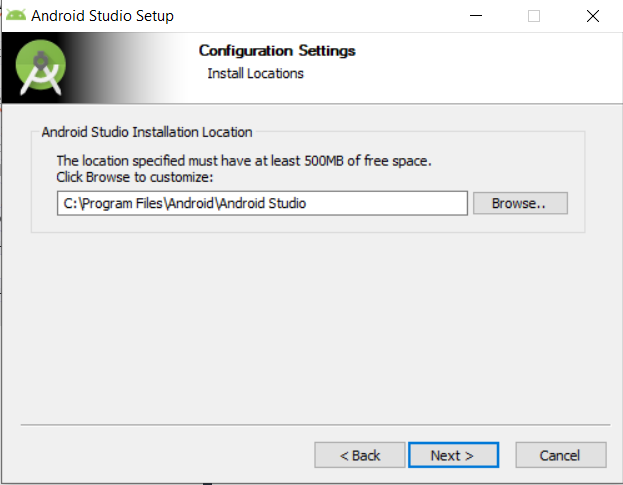
\includegraphics[width=\textwidth]{guida-installazione/android-studio/7.PNG}
    \centering
    \caption{Installazione Android Studio - Fase 7}
    \label{fig:installazione7}
\end{figure}

\begin{figure}[htbp]
    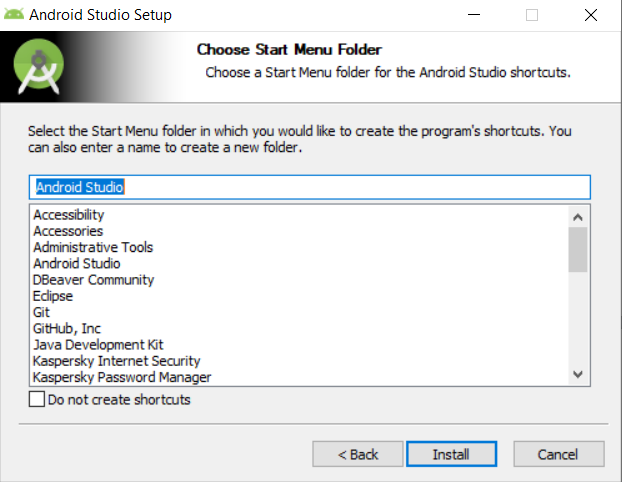
\includegraphics[width=\textwidth]{guida-installazione/android-studio/8.PNG}
    \centering
    \caption{Installazione Android Studio - Fase 8}
    \label{fig:installazione8}
\end{figure}

\begin{figure}[htbp]
    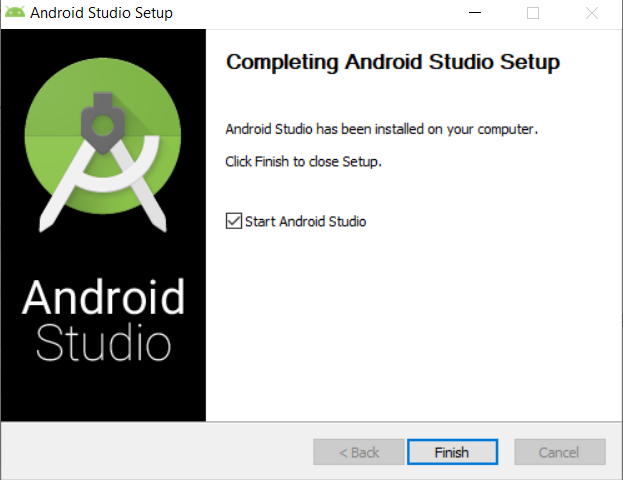
\includegraphics[width=\textwidth]{guida-installazione/android-studio/9.PNG}
    \centering
    \caption{Installazione Android Studio - Fase 9}
    \label{fig:installazione9}
\end{figure}

\clearpage

\subsection{Installazione Visual Studio Code}
\begin{enumerate}
    \item Andare sul sito \textit{https://https://code.visualstudio.com/download} e selezionare, in base al proprio sistema operativo il download corretto. In questa guida 
    è stato scelto di cliccare sul bottone relativo a \textit{Windows User installer} versione 64bit. Figura \ref{fig:installazione1VS}
    \item Aprire il file eseguibile \textit{VSCodeUserSetup.exe}. Figura \ref{fig:installazione2VS}
    \item Accettare i termi di contratto e cliccare il bottone \textit{Avanti}. Figura \ref{fig:installazione3VS}
    \item Selezionare i processi aggiuntivi desiderati e premere il bottone \textit{Avanti}. Figura \ref{fig:installazione4VS}
    \item Cliccare il bottone \textit{Installa}. Figura \ref{fig:installazione5VS}
    \item Cliccare il bottone \textit{Fine} e verrà aperto l'IDE di sviluppo Visual Studio Code. Figura \ref{fig:installazione6VS}
\end{enumerate}

\clearpage

\begin{figure}[htbp]
    \includegraphics[width=\textwidth]{guida-installazione/visual-studio/1.PNG}
    \centering
    \caption{Installazione Visual Studio Code - Fase 1}
    \label{fig:installazione1VS}
\end{figure}
\begin{figure}[htbp]
    \includegraphics[width=\textwidth]{guida-installazione/visual-studio/2.PNG}
    \centering
    \caption{Installazione Visual Studio Code - Fase 2}
    \label{fig:installazione2VS}
\end{figure}
\begin{figure}[htbp]
    \includegraphics[width=\textwidth]{guida-installazione/visual-studio/3.PNG}
    \centering
    \caption{Installazione Visual Studio Code - Fase 3}
    \label{fig:installazione3VS}
\end{figure}
\begin{figure}[htbp]
    \includegraphics[width=\textwidth]{guida-installazione/visual-studio/4.PNG}
    \centering
    \caption{Installazione Visual Studio Code - Fase 4}
    \label{fig:installazione4VS}
\end{figure}
\begin{figure}[htbp]
    \includegraphics[width=\textwidth]{guida-installazione/visual-studio/5.PNG}
    \centering
    \caption{Installazione Visual Studio Code - Fase 5}
    \label{fig:installazione5VS}
\end{figure}
\begin{figure}[htbp]
    \includegraphics[width=\textwidth]{guida-installazione/visual-studio/6.PNG}
    \centering
    \caption{Installazione Visual Studio Code - Fase 6}
    \label{fig:installazione6VS}
\end{figure}